\documentclass{article}
\usepackage{amsfonts, amsmath, amssymb, amsthm} % Math notations imported
\usepackage{enumitem}
\usepackage[margin=1in]{geometry}
\usepackage{graphicx}
\graphicspath{{./images/}} % Path to images

\newtheorem{thm}{Theorem}
\newtheorem{prop}[thm]{Proposition}
\newtheorem{cor}[thm]{Corollary}

% title information
\title{Math 181A HW7}
\author{Neo Lee}
\date{05/16/2023}

% main content
\begin{document} 

% placing title information; comment out if using fancyhdr
\maketitle 

\textbf{Problem 6.2.1}
We reject null hypothesis if the p-value is smaller than $\alpha$.
\begin{enumerate}[label={(\alph*)}]
    \item \begin{align*}
        z & = \frac{114.2-120}{18/\sqrt{25}} \approx-1.61.
    \end{align*}
    According to z-table, the p-value is $0.0537 < 0.08$. Hence, we reject $H_0$ with 92\% confidence.

    \item
    \begin{align*}
        z & = \frac{45.1-42.9}{3.2/\sqrt{16}} = 2.75.
    \end{align*}
    According to z-table, the p-value is $0.003 < \frac{0.01}{2} = 0.005$. Hence, we reject $H_0$ with 99\% confidence.

    \item
    \begin{align*}
        z & = \frac{15.8-14.2}{4.1/\sqrt{9}} \approx 1.17.
    \end{align*}
    According to z-table, the p-value is $0.121 < 0.13$. Hence, we reject $H_0$ with 87\% confidence.
\end{enumerate}
\bigbreak


\textbf{Problem 6.2.5}
Since $H_1 : \mu \neq \mu_0$ is a two-sided test, the p-value of the statistic would need to be half of that of a one-sided test for $H_1 : \mu > \mu_0$. 
Hence, $H_1 : \mu \neq \mu_0$ is more restrictive than $H_1 : \mu > \mu_0$. So, a favor of $H_1 : \mu > \mu_0$ does not necessarily mean a favor of $H_1 : \mu \neq \mu_0$.
\bigbreak


\textbf{Problem 6.2.8}
Already did.
\bigbreak


\textbf{Problem 6.2.10}
Let $H_0: \mu = 120$, $H_1: \mu > 120$, $\alpha = 0.01$.
\begin{align*}
    z & = \frac{125.2-120}{12/\sqrt{50}} \approx 3.06.
\end{align*}
According to z-table, the p-value is $0.0011 < 0.01$. Hence, we reject $H_0$ with 99\% confidence.
\bigbreak


\textbf{Problem 6.3.3}
Let $H_0: p = 0.65$, $H_1: p < 0.65$.
\begin{align*}
    z & = \frac{0.6-0.65}{\sqrt{\frac{0.65(1-0.65)}{120}}} \approx -1.15.
\end{align*}
According to z-table, the p-value is $0.125 > 0.05$. Hence, we fail to reject $H_0$ with 95\% confidence.
\bigbreak


\textbf{Problem 6.3.4}
For $\alpha = 0.14$, $z = 1.08$.
Hence, to reject $H_0$,
\begin{align*}
    z = \frac{p-0.45}{\sqrt{\frac{0.45(1-0.45)}{200}}} & > 1.08 \\
    p & > 0.488 \\
    np & > 97.6.
\end{align*}
Therefore, minimum number of success is 98.
\bigbreak


\textbf{Problem 6.3.9}
\begin{enumerate}[label={(\alph*)}]
    \item
    \begin{align*}
        \alpha & = {7\choose 0}0.25^7 + {7\choose 1}0.25^6\cdot 0.75 + {7\choose 2}0.25^5\cdot 0.75^2 + {7\choose 3}0.25^4\cdot 0.75^3 \\
        & \approx 0.071.
    \end{align*}
    
    \item \indent \\
    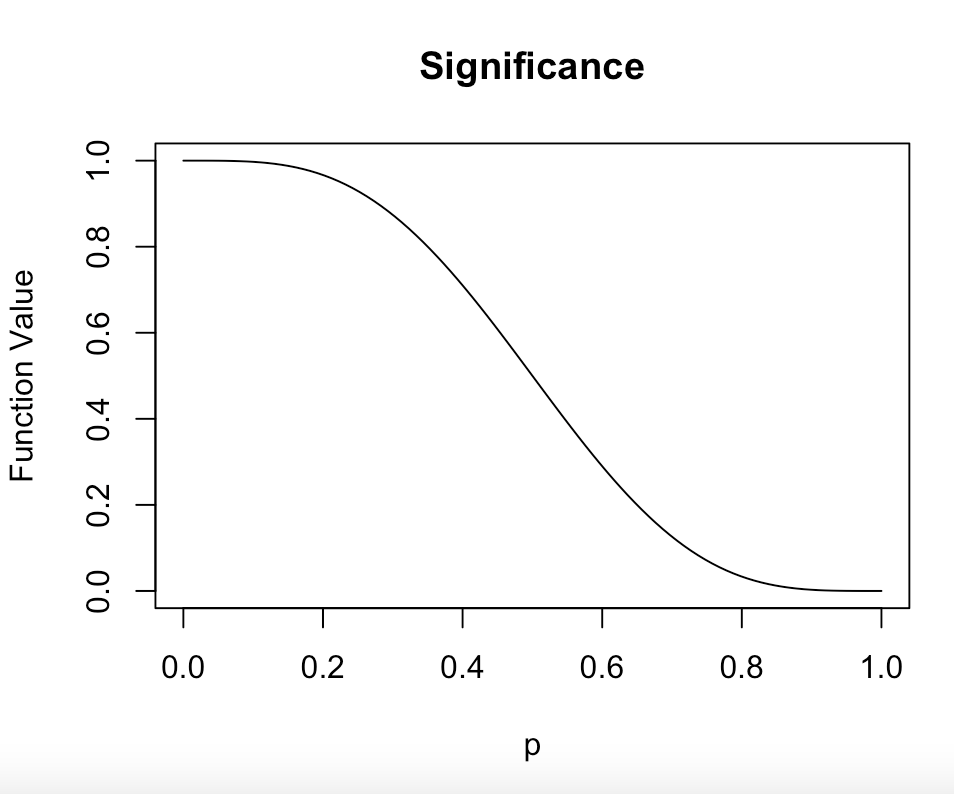
\includegraphics{graph.png}
\end{enumerate}
\bigbreak



\end{document}